% \iffalse meta-comment
% !TeX program = xelatex
% !TeX encoding = utf-8
%<*internal>
\begingroup
%</internal>
%<*install>
%%
%% This is file `l3docstrip.tex',
%% generated with the docstrip utility.
%%
%% The original source files were:
%%
%% l3docstrip.dtx  (with options: `program')
%% 
%% Copyright (C) 1990-2020 The LaTeX3 Project
%% 
%% It may be distributed and/or modified under the conditions of
%% the LaTeX Project Public License (LPPL), either version 1.3c of
%% this license or (at your option) any later version.  The latest
%% version of this license is in the file:
%% 
%%    https://www.latex-project.org/lppl.txt
%% 
%% This file is part of the "l3kernel bundle" (The Work in LPPL)
%% and all files in that bundle must be distributed together.
%% 
%% File l3dosctrip.dtx
\input docstrip %
\def\checkOption<#1{%
  \ifcase
    \ifx*#10\else \ifx/#11\else
    \ifx+#12\else \ifx-#13\else
    \ifx<#14\else \ifx @#15\else 6\fi\fi\fi\fi\fi\fi\relax
  \expandafter\starOption\or
  \expandafter\slashOption\or
  \expandafter\plusOption\or
  \expandafter\minusOption\or
  \expandafter\verbOption\or
  \expandafter\moduleOption\or
  \expandafter\doOption\fi
  #1%
}
\def\moduleOption @@=#1>#2\endLine{%
  \maybeMsg{<@@=#1>}%
  \prepareActiveModule{#1}%
}
\begingroup
  \catcode`\_ = 12 %
  \long\gdef\prepareActiveModule#1{%
    \ifx\relax#1\relax
       \let\replaceModuleInLine\empty
    \else
      \edef\replaceModuleInLine{%
        \noexpand\replaceAllIn\noexpand\inLine{@@@@}{\string aa}%
        \noexpand\replaceAllIn\noexpand\inLine{__@@}{__#1}%
        \noexpand\replaceAllIn\noexpand\inLine{_@@}{__#1}%
        \noexpand\replaceAllIn\noexpand\inLine{@@}{__#1}%
        \noexpand\replaceAllIn\noexpand\inLine{\string aa}{@@}%
      }%
    \fi
  }
\endgroup
\let\replaceModuleInLine\empty
\long\def\replaceAllIn#1#2#3{%
  \long\def\tempa##1##2#2{%
    ##2\qMark\replaceAllInAuxIII#3##1%
  }%
  \edef#1{\expandafter\replaceAllInAuxI#1\qMark#2\qStop}%
}
\def\replaceAllInAuxI{%
  \expandafter\replaceAllInAuxII\tempa\replaceAllInAuxI\empty
}
\long\def\replaceAllInAuxII#1\qMark#2{#1}
\long\def\replaceAllInAuxIII#1\qStop{}
\def\normalLine#1\endLine{%
  \maybeMsg{.}%
  \def\inLine{#1}%
  \replaceModuleInLine
  \let\do\putline@do
  \activefiles
}
\def\doOption#1>#2\endLine{%
  \maybeMsg{<#1 . >}%
  \Evaluate{#1}%
  \def\do##1##2##3{%
    \if1\Expr{##2}%
      \def\inLine{#2}%
      \replaceModuleInLine
      \StreamPut##1{\inLine}%
    \fi
  }%
  \activefiles
}
%% 
%%
%% End of file `l3docstrip.tex'.

\keepsilent
\askforoverwritefalse
\preamble
------------------------------------------------------------------------------

langsci-avm: Attribute-value matrices (AVMs) and feature structures in LaTeX3.

Copyright (C) 2020 by Felix Kopecky, Language Science Press

This work consists of the file  langsci-avm.dtx &
                                include/smallcaps-standalone.pdf.
          and the derived files langsci-avm.ins,
                                langsci-avm.pdf, 
                                langsci-avm.sty.
                                
It may be distributed and/or modified under the conditions of the
LaTeX Project Public License (LPPL), either version 1.3c of this
license or (at your option) any later version. The latest version
of this license is at <http://www.latex-project.org/lppl.txt>.

This work is ``maintained'' (per LPPL maintenance status) by
Felix Kopecky <felix.kopecky@langsci-press.org>.

The development version of the bundle can be found at

   https://github.com/langsci/langsci-avm

for those people who are interested. Pull requests are welcome.

Please report any bugs or feature requests to 

   https://github.com/langsci/langsci-avm/issues

------------------------------------------------------------------------------
\endpreamble
\declarepreamble\minimalpreamble
\endpreamble
\postamble
\endpostamble
\usedir{tex/latex/langsci-avm}
\generate{
  \file{\jobname.sty}{\from{\jobname.dtx}{package}}
}
%</install>
%<install>\endbatchfile
%<*internal>
\usepreamble\minimalpreamble
\usepostamble\defaultpostamble
\usedir{source/latex/langsci-avm}
\generate{
  \file{\jobname.ins}{\from{\jobname.dtx}{install}}
}
\endgroup
%</internal>
%<*driver>
\documentclass{l3doc}
\usepackage[linguistics]{forest}
\usepackage{langsci-avm,enumitem,url,gb4e}
\setlist[description]{font=\normalfont}
\begin{document}
  \DocInput{\jobname.dtx}
\end{document}
%</driver>
% \fi
% \title{\pkg{langsci-avm}}
% \author{Felix Kopecky\thanks{\protect\url{mailto:felix.kopecky@langsci-press.org}. 
% 		Please submit bug reports and feature requests to
% 		\protect\url{https://github.com/langsci/langsci-avm/issues}.
% 	}}
% \date{Version 0.1.0-beta -- 11th March 2020}
% \maketitle
% \frenchspacing
% \begin{documentation}
% \section{Introduction}
% \pkg{langsci-avm} is a \LaTeX3 package aimed at typesetting beautiful feature structures, also known as \emph{attribute-value matrices}, for use in linguistics. The package provides a minimal and easy to read syntax. It depends only on the \pkg{array} package and can be placed almost everywhere, in particular in footnotes or graphs and tree structures. The package is meant as an update to, and serves the same purpose as, Christopher Manning's \pkg{avm} package, but shares no code base with that package. When you come from \pkg{avm}, please see Section~\ref{sec:switching} for a quick conversion guide.
%
% To start using \pkg{langsci-avm}, place |\usepackage{langsci-avm}| in your preamble.
% 
% \subsection{Example}
% \begin{verbatim}
% \avm{
% [ ctxt & [ max-qud \\
%            sal-utt & \{ [  cat \\ 
%                           cont <ind & i> 
%                         ]
%                      \}
%           ]
% ]
% }
% \end{verbatim}
% {\centering\avm{
%     [ ctxt & [max-qud \\
%                 sal-utt & \{ [  cat\\ cont <ind & i> ]  \}\\
%                 ]
%     ]
% }\medskip\\}
% \subsection{Acknowledgements}
% Thanks to Phelype Oleinik for help on recursion and expansion with \LaTeX3. Thanks to Ahmet Bilal Özdemir and Stefan Müller for their contributions in planning and testing this package.
% 
% \section{User interface}
% \subsection{Typing structures and settings}\label{sec:options}
% 
% \begin{function}{\avm}
%   \begin{syntax}
%     \cs{avm} \oarg{options} \marg{structure}
%   \end{syntax}
%   The heart of this package and its root document comand is |\avm|. It currently runs only in text mode, but can be run in math mode if it is escaped with |$\avm$|. In the scope of the command, delimiter characters are processed to open and close (sub-)structures, as described in Section~\ref{sec:commands}. For a description of the \meta{options}, see |\avmsetup|.
% \end{function}
% 
% \begin{function}{\avmsetup}
%   \begin{syntax}
%     \cs{avmsetup} \marg{options}
%   \end{syntax}
%   \meta{options} is a comma-separated list of |key = value| settings. The \marg{options} are the same as in \cs{avm}\oarg{options}. When inserted in \cs{avm}\oarg{options}, they apply locally, and globally if given to \cs{avmsetup}. Local settings always override global ones, and you can have any feasible number of \cs{avmsetup}s in your document.
%   
%   \begin{description}[style=nextline]
%   \item[|stretch =| \meta{factor} \hfill (initially |1.15|)] Define \cs{arraystretch}, i.e. the factor of line spacing. Increasing this may be useful if there is too little vertical space between delimiters in subsequent rows.
%   
%   \item[|columnsep =| \meta{length} \hfill (initially |0.5ex|)] Define the \cs{arraycolsep}, i.e. horizontal space before and after any column. The first and second column will have |1\columnsep| to the left and right, respectively. Between the two the distance is |2\columnsep|. Using relative units (like |ex| or |em|) may be a good idea so that |columnsep| scales well with changes in font size.
%   
%   \item[|delimfactor =| \meta{factor} \hfill (initially |1000|)] Sets \cs{delimiterfactor}. The calculation for the minimum height of a delimiter is $y \cdot f /1000$, where $y$ is the height of the content and $f$ the value of  \cmd{delimfactor}. The default |1000| ensure that the delimiters' height is at least that of the structure.
%   
%   \item[|delimfall =| \meta{length} \hfill (initially |0pt|)] Controls \cs{delimitershortfall}, i.e. the maximum height that the delimiters can be shorter than the enclosed structure. The default |0pt| ensure that the delimiters are not shorter than the contents.
%   
%   \item[|attributes =| \meta{font settings} \hfill (initially |\textbackslash scshape|)] The font for attributes, i.e. the first column of each structure.
%   
%   \item[|values =| \meta{font settings} \hfill (initially |\textbackslash itshape|)] The font for values, i.e. the second column of each structure.
%   
%   \item[|types =| \meta{font settings} \hfill (initially |\textbackslash itshape|)] The font used in \cs{type} and \cs{type*}.
%   \item[|tags =| \meta{format settings} \hfill (initially |\textbackslash footnotesize|)] The font (size) used in \cs{tag} and the shortcuts \cs{1}...\cs{9}.
%   \item[|switch =| \meta{token} \hfill (initially |!|)] Define the escape token. Change this if you need to use ``!'' as a text glyph.
%   \end{description}
% \end{function}
% 
% \subsection{Commands available in the scope of \texttt{\textbackslash avm}}\label{sec:commands}
% 
% \begin{function}{[...],<...>,(...),\{...\}}
% \begin{syntax}
%     \cmd{[} \meta{structure} \cmd{]}
%     \cmd{<} \meta{structure} \cmd{>}
%     \cmd{(} \meta{structure} \cmd{)}
%     \cmd{\{} \meta{structure} \cmd{\}}
%   \end{syntax}
%   Within the scope of \cs{avm}, these delimiters create (sub-)structures that are enclosed by the respective delimiter.  Due to the special meaning that curly braces have in \LaTeX, they are the only ones that need to be run with an escape token (|\|). It is currently possible to mix delimiters, e.g. with |<|\meta{structure}|)|, but this may change in future versions.
%   
%   A \meta{structure} is basically the content of a stylised \cmd{array}: The columns are separated by \cmd{&} and a new line is entered with \cmd{\\}.
%   
%   \pkg{langsci-avm} expects your (sub-)structures to have \emph{at most two columns}, so that for every line in each (sub-)structure, there should be no more than one \cmd{&}. It is recommended to have exactly one \cmd{&} in your \meta{structure}. In the current beta version, display issues may appear in some structures if none is given.\bigskip\\
%   \noindent\begin{minipage}[c]{.5\linewidth}
% \begin{verbatim}
% \avm{
%   [ < ( \{ ... \} ) > ]
% }
% \end{verbatim}
% \end{minipage}\begin{minipage}[c]{.5\linewidth}
% \avm{
%   [ < ( \{ ... \} ) > ]
% }
% \end{minipage}\bigskip\\
% \noindent\begin{minipage}[c]{.5\linewidth}
% \begin{verbatim}
% \avm{
%   [ \{ ... \} \\
%   < ( ... ), ( ... ) > ]
% }
% \end{verbatim}
% \end{minipage}\begin{minipage}[c]{.5\linewidth}
% \avm{
%   [ \{ ... \} \\
%   < ( ... ), ( ... ) > ]
% }
% \end{minipage}
% \end{function}
% 
% \begin{function}{!...!}
% \begin{syntax}
%     \cmd{!} \meta{text} \cmd{!}
%   \end{syntax}
%   Escapes the |avm| mode so that all delimiters can be used as usual characters. If you need |!| as a regular character, see \cs{avmsetup} to change the |switch| option.
% \end{function}
% 
% \begin{function}{\tag,\1,...,\9}
%   \begin{syntax}
%    \cs{tag} \marg{identifier}
%    \cmd{\1, \2, \3, \4, \5, \6, \7, \8, \9}
%   \end{syntax}
%   \cs{tag} puts its \marg{identifier} in a box, more precisely an \cs{fbox}. Within the box, the |tags| font is applied. \cs{1}, ..., \cs{9} are shortcuts to \cs{tag} and place the respective number in the box. For example, \cs{4} is equivalent to |\tag{4}|. The shortcuts do not take any arguments.
%   
% If you want to use this command outside an AVM, you can obtain, for example, \avm{\4}, by using |\avm{\4}|, or the equivalent  |{\fboxsep.25ex\fbox{\footnotesize 4}}|.\bigskip\\   
% \noindent\begin{minipage}{.6\linewidth}
% \begin{verbatim}
% \avm{[ attr1 & \4\\
%        attr2 & \4[attr3 & val3\\
%                   attr4 & val4] ]}
%  \end{verbatim}
%  \end{minipage}\begin{minipage}{.4\linewidth}
%  \avm{[ attr1 & \4\\
% 	attr2 & \4[attr3 & val3\\
% 	attr4 & val4] ]}
%   \end{minipage}
% \end{function}
% 
% \begin{function}{\type,\type*} 
%   \begin{syntax}
%     \cs{type}\meta{*} \marg{type}
%   \end{syntax}
%   Will typeset the \meta{type} in the |types| font (roman italics by default). The starred variant \cs{type*} will span the complete (sub-)structure and \emph{can only be placed in the first column} of this structure. After the starred \cs{type*}, a |\\| is recommended, but can be omitted in ``normal'' cases.\bigskip\\   
%   \noindent\begin{minipage}{.6\linewidth}
% \begin{verbatim}
% \avm{[ \type*{A type spanning a line}
%        attr & [\type{type}] ]}
% \end{verbatim}
%   \end{minipage}\begin{minipage}{.4\linewidth}
%   	\avm{[
%   		\type*{A type spanning a line}
%   		attr & [\type{type}]
%   		]}
%   \end{minipage}
% \end{function}
% 
% \begin{function}{\punk}
% \begin{syntax}
%   \cs{punk} \marg{attribute}\marg{type}
% \end{syntax}
% Some \meta{attributes} think that the layout of the other attributes in their community leaves no space for them to express their individuality. They desire a life outside the confines of the alignment defined by the others, while still remaining a member of the matrix.
%    
% Technically, this is a line with no snapping to the column layout, but with spacing between the \meta{attribute} and \meta{type}. After \cs{punk}, a |\\| is recommended, but can be omitted in ``normal'' cases.\bigskip\\   
% \noindent\begin{minipage}{.6\linewidth}
% \begin{verbatim}
% \avm{[ attr1 & val1\\
%       \punk{a quite long attr2}{val2} ]}
%        attr3 & val3\\
%        attr4 & val4\\
% \end{verbatim}
% \end{minipage}\begin{minipage}{.4\linewidth}
%    \avm{[
%    	attr1 & val1\\
%    	\punk{a quite long attr2}{val2}
%       attr3 & val3\\
%       attr4 & val4\\
%    	]}
%    \end{minipage}
% \end{function}
% 
% \begin{function}{+}
%   In the scope of \cs{avm}, \cmd{+} comes out as ``$\oplus$''. To obtain ``+'', please use the escape mode, as in |!+!|.
% \end{function}
% 
% \section{Applications}
% 
% \subsection{Disjunctions and other relations}
% Sometimes AMVs are placed beside other content to express disjunctions or other relations. In \pkg{langsci-avm} this is done naturally:\bigskip\\
% \noindent\begin{minipage}[c]{.5\textwidth}
% \begin{verbatim}
% \avm{ [attr1 & val1\\
%        attr2 & val2\\
%        attr3 & val3] } $\lor$ 
% \avm{ [attr1' & val1'\\
%        attr2' & val2'\\
%        attr3' & val3'\\] }
% \end{verbatim}
% \end{minipage}\begin{minipage}[c]{.5\textwidth}
%  \avm{ [attr1 & val1\\
%          attr2 & val2\\
%          attr3 & val3] } $\lor$ 
%  \avm{ [attr1' & val1'\\
%         attr2' & val2'\\
%         attr3' & val3'\\] }
% \end{minipage}\bigskip\\
% \noindent\begin{minipage}[c]{.5\textwidth}
% \begin{verbatim}
% \textit{sign} $\to$ 
% \avm{ [ attribute1 & value1\\
%         attribute2 & value2\\
%         attribute3 & value3 ] }
% \end{verbatim}
% \end{minipage}\begin{minipage}[c]{.5\textwidth}
%   \textit{sign} $\to$ 
% \avm{ [ attribute1 & value1\\
% 	attribute2 & value2\\
% 	attribute3 & value3 ] }
% \end{minipage}
% 
% \subsection{Use as a vector}
% It's possible to use \pkg{langsci-avm} for feature vectors rather than matrices, as may be useful in generative grammar.\medskip\\
% \noindent\begin{minipage}[c]{.8\textwidth}
% \begin{verbatim}
% \avm[attributes=\normalfont]{[v1\\v2\\v3]}$\varphi$
% \end{verbatim}
% \end{minipage}\begin{minipage}[c]{.2\textwidth}
% \avm[attributes=\normalfont]{[v1\\v2\\v3]}$\varphi$
% \end{minipage}
% 
% \subsection{Combinations with \pkg{gb4e} and \pkg{expex}}
% 
% This package works fine with \pkg{gb4e} and its fork \pkg{langsci-gb4e}. To align the example number at the top of your structure, please use \cs{attop} from \pkg{gb4e}:\bigskip\\
% \noindent\begin{minipage}[c]{.5\textwidth}
% \begin{verbatim}
% \begin{exe}
%     \ex\attop{
%     \avm{[ attr1 & val1\\
%            attr2 & val2\\
%            attr3 & val3]}
%     }
%   \end{exe}
% \end{verbatim}
% \end{minipage}\begin{minipage}[c]{.5\textwidth}
%   \begin{exe}
% 	\ex\attop{
% 		\avm{[ attr1 & val1\\
% 			attr2 & val2\\
% 			attr3 & val3]}
% 	}
% \end{exe}
% \end{minipage}\bigskip\\
% 
% \noindent The same can be achieved with \pkg{expex} using an \emph{experimental} syntax:
% 
% \begin{verbatim}
% \ex \vtop{\strut\vskip-\baselineskip{
%   \avm{[ attr1 & val1\\
%          attr2 & val2\\
%          attr3 & val3]} 
% }}
% \xe
% \end{verbatim}
% 
% \noindent A future version of \pkg{langsci-avm} will include a more user-friendly approach. There is currently no known way of adjusting the alignment with \pkg{linguex}.
% 
% \subsection{Combinations with \pkg{forest}}
% This package also works fine with \pkg{forest}. As per the \pkg{forest} documentation, it is recommended to protect any \cs{avm}-statements with |{}| in nodes:\bigskip\\
% \noindent\begin{minipage}[c]{.6\textwidth}
% \begin{verbatim}
% \begin{forest}
%  [A [B] [{\avm{[attr1 & val1\\
%                 attr2 & val2\\
%                 attr3 & val3]}} ] ]
% \end{forest}
% \end{verbatim}
% \end{minipage}\begin{minipage}[c]{.4\textwidth}
% \begin{forest}
% 	[A [B] [{\avm{[attr1 & val1\\
% 			attr2 & val2\\
% 			attr3 & val3]}} ] ]
% \end{forest}
% \end{minipage}
% 
% \subsection{Switching from Christopher Manning's \pkg{avm} package}\label{sec:switching}
% Switching from \pkg{avm} to \pkg{langsci-avm} will require some, though hopefully minimal, changes to the code. In particular, the ``active mode'' has disappeared, there is now a single way of sorting (see \cs{type}), and tags are now produced without |@| (\cs{4} instead of \cmd{@4}, etc.). Please refer to Section~\ref{sec:caveats} for features known from \pkg{avm} that are not yet available in \pkg{langsci-avm}.
% 
% \subsection{Tweaking the \texttt{attribute} font with with \pkg{fontspec}}
% The attributes in your structure are usually type set in \textsc{small caps}. That means that your input should usually be lowercase, unless capitals along small capitals in that attribute's description make sense. Some fonts also provide ``old style'' figures (also known as ``text'' or ``medieval'' figures). Those can be enabled with \pkg{fontspec}'s |Numbers=OldStyle| feature. 
% 
% 
% \textit{The following example is output in Libertinus, since the font for this documentation does not support the necessary font features.}\bigskip\\
% \begin{minipage}[c]{.7\linewidth}
% \begin{verbatim}
% % Preamble 
%  \usepackage{fontspec}
%  \usepackage{libertinus}
% % Document
%  \avm[attributes={\addfontfeatures{
%       Numbers=OldStyle,
%       Letters=SmallCaps}
%       } 
%       ] { [attr1 & val2] }
% 	\end{verbatim}
% \end{minipage}\begin{minipage}[c]{.3\linewidth}
% 	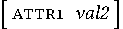
\includegraphics{include/smallcaps-standalone.pdf}
% \end{minipage}
% 
% \subsection{Spanning both columns}
% You can use the \pkg{multicol} package to span both columns in a (sub-)structure. Please remember that every structure has two columns, so the only sensible usage is 
% 
% \begin{verbatim}
% \multicolumn{2}{l}{...}
% \end{verbatim}
% 
% \noindent but only in the first column of a (sub-)structure. For a special usage case, see \cs{type} and \cs{type*} (which do not depend on \pkg{multicol}).
% 
% \section{Caveats and planned features}\label{sec:caveats}
% \begin{enumerate}
% \item There are currently no error messages. If you do not receive the intended output, please make sure that your code fits the syntax described in this documentation. If your code is fine but the output is not, please submit a bug report or feature request at \url{https://github.com/langsci/langsci-avm/issues}.
% \item The package currently assumes that it is called in text mode.
% \item[] These features are planned for the future:
% \item A check whether the delimiters are balanced, i.e. whether all (sub-)structures are closed by a \verb+]+, \verb+}+, etc.
% \item Introduce the ability to draw (curved) lines between structures and elements.
% \item Improve the appearance of angle brackets so that they vertically span the complete structure they enclose, maybe using \pkg{scalerel}.
% \end{enumerate}
% 
% \section{Feedback and bug reports}
% Comments, usage reports, and feature requests are welcome! Please open an issue for any of these at \url{https://github.com/langsci/langsci-avm/issues}, or write to me at \url{mailto:felix.kopecky@langsci-press.org} if you feel the need for a feature not listed here, big or small.
% \end{documentation}
% 
% \begin{implementation}
% 
% \section{Implementation}
%    \begin{macrocode}
%<*package>
%    \end{macrocode}
%    \begin{macrocode}
%<@@=avm>
%    \end{macrocode}
%    \begin{macrocode}
\RequirePackage{xparse,array}
%    \end{macrocode}
%
%    \begin{macrocode}
\ProvidesExplPackage {langsci-avm} 
  {2020-03-11} {0.1.0-beta}
  {AVMs and feature structures in LaTeX3}
%    \end{macrocode}
%    \begin{macro}{\avm}
% This document command initialises an AVM. The first, optional argumet is a key-value list of settings (see \cs{keys_define:nn} below) and the second is the AVM itself, given in the syntax described in this documentation.
% 
% \cs{avm} enters a group so that keys- and macro-assignemts remain local. It then initialises the commands and shortcuts made locally available, sets its mode to |true| and assigns the keys as given in the optional argument (if any). After the wrapper \cs{avm_wrap:n} is called, the group is closed.
%
%    \begin{macrocode}
\NewDocumentCommand{\avm}{ O{} +m }
  {
    \c_group_begin_token
    \__avm_initialise_document_commands:
    \bool_set_true:N \l__avm_mode_bool
    \keys_set:nn { avm } { #1 }
    \__avm_wrap:n { #2 }
    \c_group_end_token
  }
%    \end{macrocode}
%    \end{macro}
%
%    \begin{macro}{\avmsetup}
% Forward the key-value settings given as the optional argument to \cs{avm} to the keys defined in |\keys_define:nn { avm }|. For the meaning of these keys and initial values, see Section~\ref{sec:options}.
% 
%    \begin{macrocode}
\NewDocumentCommand{\avmsetup}{ m } 
  { \keys_set:nn { avm } { #1 } }

\keys_define:nn { avm }
  {
    stretch .code:n        = {\def\arraystretch{#1}},
    stretch .initial:n     = {1.15},
    columnsep .dim_set:N   = \arraycolsep,
    columnsep .initial:n   = {.5ex},
    delimfactor .int_set:N = \delimiterfactor,
    delimfactor .initial:n = {1000},
    delimfall .dim_set:N   = \delimitershortfall,
    delimfall .initial:n   = {0pt},
    attributes .code:n     = {\cs_set:Nn \__avm_font_attribute: {#1}},
    attributes .initial:n  = {\scshape},
    types .code:n          = {\cs_set:Nn \__avm_font_type: {#1}},
    types .initial:n       = {\itshape},
    values .code:n         = {\cs_set:Nn \__avm_font_value: {#1}},
    values .initial:n      = {\itshape},
    tags .code:n           = {\cs_set:Nn \__avm_font_tag: {#1}},
    tags .initial:n        = {\footnotesize},  
    switch .code:n         = {\tl_set:Nn \__avm_mode_switch_character {#1}},
    switch .initial:n      = { ! }
  }
%    \end{macrocode}
%    \end{macro}
  
%    \begin{variable}{\l__avm_math_bool, \l__avm_mode_bool, \l__avm_parens_tracker}
% We need an auxiliary variable to store the current mode. The math mode boolean is already created, but it will have an effect only in a later version which will include a check whether \cs{avm} is called in math mode. \cs{l__avm_parens_tracker} is a stack for a future check whether the delimiters given to \cs{avm} are balanced.
%    \begin{macrocode}
\bool_new:N \l__avm_math_bool
\bool_new:N \l__avm_mode_bool
\seq_new:N \l__avm_parens_tracker
%    \end{macrocode}
%    \end{variable}

%    \begin{macro}[int]{\seq_set_split:NVn}
% In preparation for \cs{avm_wrap:n}, we need to split the user input at each occurrence of the escape character. Since the character is given in a variable, we need a variant of the sequence splitter that takes the \emph{evaluation} of the variable, rather than the variable itself, as its second argument.
%    \begin{macrocode}
\cs_generate_variant:Nn \seq_set_split:Nnn { NVn }
%    \end{macrocode}
%    \end{macro}


%    \begin{macro}[int]{\__avm_module_begin:,\__avm_module_end:,etc.}
% The replacement instructions for \cs{__avm_parse:n}
%    \begin{macrocode}
\cs_new:Nn \__avm_module_begin: 
  { 
    \begin{array}{ 
      >{\c_math_toggle_token\normalfont\__avm_font_attribute:}l
      <\c_math_toggle_token
      >{\c_math_toggle_token\normalfont\__avm_font_value:}l
      <\c_math_toggle_token} 
  }
\cs_new:Nn \__avm_module_end:
  { \end{array} }
\cs_new:Nn \__avm_replace_lbrace: 
  { 
    \__avm_parse_output:nw 
      { \c_math_toggle_token\left\lbrace\__avm_module_begin: } 
  }
\cs_new:Nn \__avm_replace_rbrace: 
  { 
    \__avm_parse_output:nw 
      { \__avm_module_end:\right\rbrace\c_math_toggle_token  } 
  }
\cs_new:Nn \__avm_replace_lbrack: 
  { 
    \__avm_parse_output:nw 
      { \c_math_toggle_token\left\lbrack\__avm_module_begin: } 
  }     
\cs_new:Nn \__avm_replace_rbrack: 
  { 
    \__avm_parse_output:nw 
      { \__avm_module_end:\right\rbrack\c_math_toggle_token } 
  }
\cs_new:Nn \__avm_replace_lparen: 
  { 
    \__avm_parse_output:nw 
      { \c_math_toggle_token\left(\__avm_module_begin: } 
  } 
\cs_new:Nn \__avm_replace_rparen: 
  { 
    \__avm_parse_output:nw 
      { \__avm_module_end:\right)\c_math_toggle_token  } 
  } 
\cs_new:Nn \__avm_replace_langle: 
  { 
    \__avm_parse_output:nw 
      { \c_math_toggle_token\left<\__avm_module_begin: } 
  } 
\cs_new:Nn \__avm_replace_rangle: 
  { 
    \__avm_parse_output:nw 
      { \__avm_module_end:\right>\c_math_toggle_token  } 
  }
\cs_new:Nn \__avm_replace_plus:
  { 
    \__avm_parse_output:nw { \ensuremath { \oplus } } 
  }
%    \end{macrocode}
%    \end{macro}

%    \begin{macro}{\tag,\type,\punk}
%    \begin{macrocode}
\cs_new:Npn \__avm_controls_tag:n #1 
  { \fboxsep.25ex\fbox{\normalfont\__avm_font_tag: #1} } 
\cs_new:Npn \__avm_controls_type:n #1 
  {\normalfont\__avm_font_type: #1}
\cs_new_protected:Npn \__avm_controls_type_starred:n #1 
  {
    \normalfont\__avm_font_type: #1\span                                                
    \peek_meaning_ignore_spaces:NTF \\ {} {\\} 
  }
\cs_new_protected:Npn \__avm_controls_punk:nn #1 #2 
  {  
     \normalfont\c_group_begin_token\__avm_font_attribute:#1%
     \c_group_end_token\hspace{2\arraycolsep}%
     \c_group_begin_token\__avm_font_type: #2\c_group_end_token%
     \span\peek_meaning_ignore_spaces:NTF \\ {} {\\}                                               
  }

\cs_new:Nn \__avm_initialise_document_commands: 
  {
    \cs_if_exist:NTF \tag 
      {  \RenewDocumentCommand{\tag}{m}{ \__avm_controls_tag:n {##1} } }
      {  \NewDocumentCommand{\tag}{m}{   \__avm_controls_tag:n {##1} } }
    \cs_if_exist:NTF \1   
      {  \RenewDocumentCommand{\1}{}{    \__avm_controls_tag:n {1} } }
      {  \NewDocumentCommand{\1}{}{      \__avm_controls_tag:n {1} } }
    \cs_if_exist:NTF \2
      {  \RenewDocumentCommand{\2}{}{    \__avm_controls_tag:n {2} } }
      {  \NewDocumentCommand{\2}{}{      \__avm_controls_tag:n {2} } }
    \cs_if_exist:NTF \3
      {  \RenewDocumentCommand{\3}{}{    \__avm_controls_tag:n {3} } }
      {  \NewDocumentCommand{\3}{}{      \__avm_controls_tag:n {3} } }
    \cs_if_exist:NTF \4
      {  \RenewDocumentCommand{\4}{}{    \__avm_controls_tag:n {4} } }
      {  \NewDocumentCommand{\4}{}{      \__avm_controls_tag:n {4} } }
    \cs_if_exist:NTF \5
      {  \RenewDocumentCommand{\5}{}{    \__avm_controls_tag:n {5} } }
      {  \NewDocumentCommand{\5}{}{      \__avm_controls_tag:n {5} } }
    \cs_if_exist:NTF \6
      {  \RenewDocumentCommand{\6}{}{    \__avm_controls_tag:n {6} } }
      {  \NewDocumentCommand{\6}{}{      \__avm_controls_tag:n {6} } }
    \cs_if_exist:NTF \7
      {  \RenewDocumentCommand{\7}{}{    \__avm_controls_tag:n {7} } }
      {  \NewDocumentCommand{\7}{}{      \__avm_controls_tag:n {7} } }
    \cs_if_exist:NTF \8
      {  \RenewDocumentCommand{\8}{}{    \__avm_controls_tag:n {8} } }
      {  \NewDocumentCommand{\8}{}{      \__avm_controls_tag:n {8} } }
    \cs_if_exist:NTF \9
      {  \RenewDocumentCommand{\9}{}{    \__avm_controls_tag:n {9} } }
      {  \NewDocumentCommand{\9}{}{      \__avm_controls_tag:n {9} } }
    \cs_if_exist:NTF \type 
      {  \RenewDocumentCommand{\type}{s m}
        {  
          \IfBooleanTF { ##1 } 
            {  \__avm_controls_type_starred:n {##2}  }
            {  \__avm_controls_type:n {##2} }
         } 
       }
       {  \NewDocumentCommand{\type}{s m}
         {
           \IfBooleanTF { ##1 }
             {  \__avm_controls_type_starred:n {##2}  }
             {  \__avm_controls_type:n {##2}  }
          } 
        }
    \cs_if_exist:NTF \punk 
      {  \RenewDocumentCommand{\punk}{m m}
        { \__avm_controls_punk:nn {##1}{##2} } }
      {  \NewDocumentCommand{\punk}{m m}
        {  \__avm_controls_punk:nn {##1}{##2} } }
  }
%    \end{macrocode}
%    \end{macro}

%    \begin{macro}{\__avm_wrap:n}
% The wrapper that first splits the input to \cs{avm} at each occurrence of \cs{__avm_mode_switch_character} and then inverses \cs{l__avm_mode_bool}. It then calls the parser (\cs{__avm_parse:n}) for each splitted sequence. This wrapping is necessary because there is no known expandable way to switch a boolean.
%    \begin{macrocode}
\cs_new_protected:Npn \__avm_wrap:n #1
  {
    \seq_set_split:NVn \l__avm_wrapper_seq 
    \__avm_mode_switch_character { #1 }
    \seq_map_inline:Nn \l__avm_wrapper_seq 
      {  
        \exp_args:No \exp_not:o 
          {  \__avm_parse:n {##1} }  
        \bool_set_inverse:N \l__avm_mode_bool 
      }
  }
%    \end{macrocode}
%    \end{macro}

%    \begin{macro}{\__avm_parse:n}
% Finnaly, the parser. It is build on \cs{@@_act:NNNnn} from \cmd{l3tl} (see the sub-section \emph{Token by token changes}). Many thanks to Phelype Oleinik for help on this, and in particular on help with expansion. 
%    \begin{macrocode}
\cs_new:Npn \__avm_parse:n #1
  {
      \exp:w
      \group_align_safe_begin:
        \__avm_parse_loop:w #1 
        \q_recursion_tail \q_recursion_stop 
        \__avm_result:n { }
  }

\cs_new:Npn \__avm_end:w \__avm_result:n #1
  {
    \group_align_safe_end:
    \exp_end:
    #1
  }

\cs_new:Npn \__avm_parse_loop:w #1 \q_recursion_stop
  {
    \tl_if_head_is_N_type:nTF {#1}
      {
        \__avm_N_type:N #1 \q_recursion_stop 
      }
      {
        \tl_if_head_is_group:nTF {#1}
          { \__avm_replace_group:nw #1 \q_recursion_stop }
          { \__avm_replace_space:w #1 \q_recursion_stop }
      }
  }
  
\cs_new:Npn \__avm_N_type:N #1
  {
    \quark_if_recursion_tail_stop_do:Nn #1 { \__avm_end:w }
    \bool_if:NTF \l__avm_mode_bool 
      { \__avm_replace:N #1 } 
      { \__avm_replace_none:N #1 } 
  }
  
\cs_new:Npn \__avm_replace_none:N #1 
  { 
    \__avm_parse_output:nw {#1}
  }

\cs_new:Npn \__avm_replace:N #1
  {
    \str_case:nnF {#1}
      {
        { +  }{ \__avm_replace_plus: }
        { [  }{ \__avm_replace_lbrack: }
        { ]  }{ \__avm_replace_rbrack: }
        { (  }{ \__avm_replace_lparen: }
        { )  }{ \__avm_replace_rparen: }
        { \{ }{ \__avm_replace_lbrace: }        
        { \} }{ \__avm_replace_rbrace: }                
        { <  }{ \__avm_replace_langle: } 
        { >  }{ \__avm_replace_rangle: } 
      }
      { \__avm_replace_none:N #1 }
  }

\cs_new:Npn \__avm_replace_group:nw #1
  { \exp_args:NNo \exp_args:No \__avm_replace_group:n { \__avm_parse:n {#1} } }

\cs_new:Npn \__avm_replace_group:n #1 { \__avm_parse_output:nw { {#1} } }

\exp_last_unbraced:NNo
\cs_new:Npn \__avm_replace_space:w \c_space_tl { \__avm_parse_output:nw { ~ } }

\cs_new:Npn \__avm_parse_output:nw #1 #2 \q_recursion_stop \__avm_result:n #3
  { \__avm_parse_loop:w #2 \q_recursion_stop \__avm_result:n {#3  #1 } }
%    \end{macrocode}
%    \end{macro}
%    \begin{macrocode}
%</package>
%    \end{macrocode}
%
% \end{implementation}

% \PrintIndex
